\documentclass{report}

%%%%%%%%%%%%%%%%%%%%%%%%%%%%%%%%%
% PACKAGE IMPORTS
%%%%%%%%%%%%%%%%%%%%%%%%%%%%%%%%%


\usepackage[tmargin=2cm,rmargin=1in,lmargin=1in,margin=0.85in,bmargin=2cm,footskip=.2in]{geometry}
\usepackage{amsmath,amsfonts,amsthm,amssymb,mathtools}
\usepackage[varbb]{newpxmath}
\usepackage{xfrac}
\usepackage[makeroom]{cancel}
\usepackage{mathtools}
\usepackage{bookmark}
\usepackage{enumitem}
\usepackage{hyperref,theoremref}
\hypersetup{
	pdftitle={Assignment},
	colorlinks=true, linkcolor=doc!90,
	bookmarksnumbered=true,
	bookmarksopen=true
}
\usepackage[most,many,breakable]{tcolorbox}
\usepackage{xcolor}
\usepackage{varwidth}
\usepackage{varwidth}
\usepackage{etoolbox}
%\usepackage{authblk}
\usepackage{nameref}
\usepackage{multicol,array}
\usepackage{tikz-cd}
\usepackage[ruled,vlined,linesnumbered]{algorithm2e}
\usepackage{comment} % enables the use of multi-line comments (\ifx \fi) 
\usepackage{import}
\usepackage{xifthen}
\usepackage{pdfpages}
\usepackage{transparent}

\newcommand\mycommfont[1]{\footnotesize\ttfamily\textcolor{blue}{#1}}
\SetCommentSty{mycommfont}
\newcommand{\incfig}[1]{%
    \def\svgwidth{\columnwidth}
    \import{./figures/}{#1.pdf_tex}
}

\usepackage{tikzsymbols}
\renewcommand\qedsymbol{$\Laughey$}


%\usepackage{import}
%\usepackage{xifthen}
%\usepackage{pdfpages}
%\usepackage{transparent}


%%%%%%%%%%%%%%%%%%%%%%%%%%%%%%
% SELF MADE COLORS
%%%%%%%%%%%%%%%%%%%%%%%%%%%%%%



\definecolor{myg}{RGB}{56, 140, 70}
\definecolor{myb}{RGB}{45, 111, 177}
\definecolor{myr}{RGB}{199, 68, 64}
\definecolor{mytheorembg}{HTML}{F2F2F9}
\definecolor{mytheoremfr}{HTML}{00007B}
\definecolor{mylenmabg}{HTML}{FFFAF8}
\definecolor{mylenmafr}{HTML}{983b0f}
\definecolor{mypropbg}{HTML}{f2fbfc}
\definecolor{mypropfr}{HTML}{191971}
\definecolor{myexamplebg}{HTML}{F2FBF8}
\definecolor{myexamplefr}{HTML}{88D6D1}
\definecolor{myexampleti}{HTML}{2A7F7F}
\definecolor{mydefinitbg}{HTML}{E5E5FF}
\definecolor{mydefinitfr}{HTML}{3F3FA3}
\definecolor{notesgreen}{RGB}{0,162,0}
\definecolor{myp}{RGB}{197, 92, 212}
\definecolor{mygr}{HTML}{2C3338}
\definecolor{myred}{RGB}{127,0,0}
\definecolor{myyellow}{RGB}{169,121,69}
\definecolor{myexercisebg}{HTML}{F2FBF8}
\definecolor{myexercisefg}{HTML}{88D6D1}


%%%%%%%%%%%%%%%%%%%%%%%%%%%%
% TCOLORBOX SETUPS
%%%%%%%%%%%%%%%%%%%%%%%%%%%%

\setlength{\parindent}{1cm}
%================================
% THEOREM BOX
%================================

\tcbuselibrary{theorems,skins,hooks}
\newtcbtheorem[number within=section]{Theorem}{Theorem}
{%
	enhanced,
	breakable,
	colback = mytheorembg,
	frame hidden,
	boxrule = 0sp,
	borderline west = {2pt}{0pt}{mytheoremfr},
	sharp corners,
	detach title,
	before upper = \tcbtitle\par\smallskip,
	coltitle = mytheoremfr,
	fonttitle = \bfseries\sffamily,
	description font = \mdseries,
	separator sign none,
	segmentation style={solid, mytheoremfr},
}
{th}

\tcbuselibrary{theorems,skins,hooks}
\newtcbtheorem[number within=chapter]{theorem}{Theorem}
{%
	enhanced,
	breakable,
	colback = mytheorembg,
	frame hidden,
	boxrule = 0sp,
	borderline west = {2pt}{0pt}{mytheoremfr},
	sharp corners,
	detach title,
	before upper = \tcbtitle\par\smallskip,
	coltitle = mytheoremfr,
	fonttitle = \bfseries\sffamily,
	description font = \mdseries,
	separator sign none,
	segmentation style={solid, mytheoremfr},
}
{th}


\tcbuselibrary{theorems,skins,hooks}
\newtcolorbox{Theoremcon}
{%
	enhanced
	,breakable
	,colback = mytheorembg
	,frame hidden
	,boxrule = 0sp
	,borderline west = {2pt}{0pt}{mytheoremfr}
	,sharp corners
	,description font = \mdseries
	,separator sign none
}

%================================
% Corollery
%================================
\tcbuselibrary{theorems,skins,hooks}
\newtcbtheorem[number within=section]{Corollary}{Corollary}
{%
	enhanced
	,breakable
	,colback = myp!10
	,frame hidden
	,boxrule = 0sp
	,borderline west = {2pt}{0pt}{myp!85!black}
	,sharp corners
	,detach title
	,before upper = \tcbtitle\par\smallskip
	,coltitle = myp!85!black
	,fonttitle = \bfseries\sffamily
	,description font = \mdseries
	,separator sign none
	,segmentation style={solid, myp!85!black}
}
{th}
\tcbuselibrary{theorems,skins,hooks}
\newtcbtheorem[number within=chapter]{corollary}{Corollary}
{%
	enhanced
	,breakable
	,colback = myp!10
	,frame hidden
	,boxrule = 0sp
	,borderline west = {2pt}{0pt}{myp!85!black}
	,sharp corners
	,detach title
	,before upper = \tcbtitle\par\smallskip
	,coltitle = myp!85!black
	,fonttitle = \bfseries\sffamily
	,description font = \mdseries
	,separator sign none
	,segmentation style={solid, myp!85!black}
}
{th}


%================================
% LENMA
%================================

\tcbuselibrary{theorems,skins,hooks}
\newtcbtheorem[number within=section]{Lenma}{Lenma}
{%
	enhanced,
	breakable,
	colback = mylenmabg,
	frame hidden,
	boxrule = 0sp,
	borderline west = {2pt}{0pt}{mylenmafr},
	sharp corners,
	detach title,
	before upper = \tcbtitle\par\smallskip,
	coltitle = mylenmafr,
	fonttitle = \bfseries\sffamily,
	description font = \mdseries,
	separator sign none,
	segmentation style={solid, mylenmafr},
}
{th}

\tcbuselibrary{theorems,skins,hooks}
\newtcbtheorem[number within=chapter]{lenma}{Lenma}
{%
	enhanced,
	breakable,
	colback = mylenmabg,
	frame hidden,
	boxrule = 0sp,
	borderline west = {2pt}{0pt}{mylenmafr},
	sharp corners,
	detach title,
	before upper = \tcbtitle\par\smallskip,
	coltitle = mylenmafr,
	fonttitle = \bfseries\sffamily,
	description font = \mdseries,
	separator sign none,
	segmentation style={solid, mylenmafr},
}
{th}


%================================
% PROPOSITION
%================================

\tcbuselibrary{theorems,skins,hooks}
\newtcbtheorem[number within=section]{Prop}{Proposition}
{%
	enhanced,
	breakable,
	colback = mypropbg,
	frame hidden,
	boxrule = 0sp,
	borderline west = {2pt}{0pt}{mypropfr},
	sharp corners,
	detach title,
	before upper = \tcbtitle\par\smallskip,
	coltitle = mypropfr,
	fonttitle = \bfseries\sffamily,
	description font = \mdseries,
	separator sign none,
	segmentation style={solid, mypropfr},
}
{th}

\tcbuselibrary{theorems,skins,hooks}
\newtcbtheorem[number within=chapter]{prop}{Proposition}
{%
	enhanced,
	breakable,
	colback = mypropbg,
	frame hidden,
	boxrule = 0sp,
	borderline west = {2pt}{0pt}{mypropfr},
	sharp corners,
	detach title,
	before upper = \tcbtitle\par\smallskip,
	coltitle = mypropfr,
	fonttitle = \bfseries\sffamily,
	description font = \mdseries,
	separator sign none,
	segmentation style={solid, mypropfr},
}
{th}


%================================
% CLAIM
%================================

\tcbuselibrary{theorems,skins,hooks}
\newtcbtheorem[number within=section]{claim}{Claim}
{%
	enhanced
	,breakable
	,colback = myg!10
	,frame hidden
	,boxrule = 0sp
	,borderline west = {2pt}{0pt}{myg}
	,sharp corners
	,detach title
	,before upper = \tcbtitle\par\smallskip
	,coltitle = myg!85!black
	,fonttitle = \bfseries\sffamily
	,description font = \mdseries
	,separator sign none
	,segmentation style={solid, myg!85!black}
}
{th}



%================================
% Exercise
%================================

\tcbuselibrary{theorems,skins,hooks}
\newtcbtheorem[number within=section]{Exercise}{Exercise}
{%
	enhanced,
	breakable,
	colback = myexercisebg,
	frame hidden,
	boxrule = 0sp,
	borderline west = {2pt}{0pt}{myexercisefg},
	sharp corners,
	detach title,
	before upper = \tcbtitle\par\smallskip,
	coltitle = myexercisefg,
	fonttitle = \bfseries\sffamily,
	description font = \mdseries,
	separator sign none,
	segmentation style={solid, myexercisefg},
}
{th}

\tcbuselibrary{theorems,skins,hooks}
\newtcbtheorem[number within=chapter]{exercise}{Exercise}
{%
	enhanced,
	breakable,
	colback = myexercisebg,
	frame hidden,
	boxrule = 0sp,
	borderline west = {2pt}{0pt}{myexercisefg},
	sharp corners,
	detach title,
	before upper = \tcbtitle\par\smallskip,
	coltitle = myexercisefg,
	fonttitle = \bfseries\sffamily,
	description font = \mdseries,
	separator sign none,
	segmentation style={solid, myexercisefg},
}
{th}

%================================
% EXAMPLE BOX
%================================

\newtcbtheorem[number within=section]{Example}{Example}
{%
	colback = myexamplebg
	,breakable
	,colframe = myexamplefr
	,coltitle = myexampleti
	,boxrule = 1pt
	,sharp corners
	,detach title
	,before upper=\tcbtitle\par\smallskip
	,fonttitle = \bfseries
	,description font = \mdseries
	,separator sign none
	,description delimiters parenthesis
}
{ex}

\newtcbtheorem[number within=chapter]{example}{Example}
{%
	colback = myexamplebg
	,breakable
	,colframe = myexamplefr
	,coltitle = myexampleti
	,boxrule = 1pt
	,sharp corners
	,detach title
	,before upper=\tcbtitle\par\smallskip
	,fonttitle = \bfseries
	,description font = \mdseries
	,separator sign none
	,description delimiters parenthesis
}
{ex}

%================================
% DEFINITION BOX
%================================

\newtcbtheorem[number within=section]{Definition}{Definition}{enhanced,
	before skip=2mm,after skip=2mm, colback=red!5,colframe=red!80!black,boxrule=0.5mm,
	attach boxed title to top left={xshift=1cm,yshift*=1mm-\tcboxedtitleheight}, varwidth boxed title*=-3cm,
	boxed title style={frame code={
					\path[fill=tcbcolback]
					([yshift=-1mm,xshift=-1mm]frame.north west)
					arc[start angle=0,end angle=180,radius=1mm]
					([yshift=-1mm,xshift=1mm]frame.north east)
					arc[start angle=180,end angle=0,radius=1mm];
					\path[left color=tcbcolback!60!black,right color=tcbcolback!60!black,
						middle color=tcbcolback!80!black]
					([xshift=-2mm]frame.north west) -- ([xshift=2mm]frame.north east)
					[rounded corners=1mm]-- ([xshift=1mm,yshift=-1mm]frame.north east)
					-- (frame.south east) -- (frame.south west)
					-- ([xshift=-1mm,yshift=-1mm]frame.north west)
					[sharp corners]-- cycle;
				},interior engine=empty,
		},
	fonttitle=\bfseries,
	title={#2},#1}{def}
\newtcbtheorem[number within=chapter]{definition}{Definition}{enhanced,
	before skip=2mm,after skip=2mm, colback=red!5,colframe=red!80!black,boxrule=0.5mm,
	attach boxed title to top left={xshift=1cm,yshift*=1mm-\tcboxedtitleheight}, varwidth boxed title*=-3cm,
	boxed title style={frame code={
					\path[fill=tcbcolback]
					([yshift=-1mm,xshift=-1mm]frame.north west)
					arc[start angle=0,end angle=180,radius=1mm]
					([yshift=-1mm,xshift=1mm]frame.north east)
					arc[start angle=180,end angle=0,radius=1mm];
					\path[left color=tcbcolback!60!black,right color=tcbcolback!60!black,
						middle color=tcbcolback!80!black]
					([xshift=-2mm]frame.north west) -- ([xshift=2mm]frame.north east)
					[rounded corners=1mm]-- ([xshift=1mm,yshift=-1mm]frame.north east)
					-- (frame.south east) -- (frame.south west)
					-- ([xshift=-1mm,yshift=-1mm]frame.north west)
					[sharp corners]-- cycle;
				},interior engine=empty,
		},
	fonttitle=\bfseries,
	title={#2},#1}{def}



%================================
% Solution BOX
%================================

\makeatletter
\newtcbtheorem{question}{Question}{enhanced,
	breakable,
	colback=white,
	colframe=myb!80!black,
	attach boxed title to top left={yshift*=-\tcboxedtitleheight},
	fonttitle=\bfseries,
	title={#2},
	boxed title size=title,
	boxed title style={%
			sharp corners,
			rounded corners=northwest,
			colback=tcbcolframe,
			boxrule=0pt,
		},
	underlay boxed title={%
			\path[fill=tcbcolframe] (title.south west)--(title.south east)
			to[out=0, in=180] ([xshift=5mm]title.east)--
			(title.center-|frame.east)
			[rounded corners=\kvtcb@arc] |-
			(frame.north) -| cycle;
		},
	#1
}{def}
\makeatother

%================================
% SOLUTION BOX
%================================

\makeatletter
\newtcolorbox{solution}{enhanced,
	breakable,
	colback=white,
	colframe=myg!80!black,
	attach boxed title to top left={yshift*=-\tcboxedtitleheight},
	title=Solution,
	boxed title size=title,
	boxed title style={%
			sharp corners,
			rounded corners=northwest,
			colback=tcbcolframe,
			boxrule=0pt,
		},
	underlay boxed title={%
			\path[fill=tcbcolframe] (title.south west)--(title.south east)
			to[out=0, in=180] ([xshift=5mm]title.east)--
			(title.center-|frame.east)
			[rounded corners=\kvtcb@arc] |-
			(frame.north) -| cycle;
		},
}
\makeatother

%================================
% Question BOX
%================================

\makeatletter
\newtcbtheorem{qstion}{Question}{enhanced,
	breakable,
	colback=white,
	colframe=mygr,
	attach boxed title to top left={yshift*=-\tcboxedtitleheight},
	fonttitle=\bfseries,
	title={#2},
	boxed title size=title,
	boxed title style={%
			sharp corners,
			rounded corners=northwest,
			colback=tcbcolframe,
			boxrule=0pt,
		},
	underlay boxed title={%
			\path[fill=tcbcolframe] (title.south west)--(title.south east)
			to[out=0, in=180] ([xshift=5mm]title.east)--
			(title.center-|frame.east)
			[rounded corners=\kvtcb@arc] |-
			(frame.north) -| cycle;
		},
	#1
}{def}
\makeatother

\newtcbtheorem[number within=chapter]{wconc}{Wrong Concept}{
	breakable,
	enhanced,
	colback=white,
	colframe=myr,
	arc=0pt,
	outer arc=0pt,
	fonttitle=\bfseries\sffamily\large,
	colbacktitle=myr,
	attach boxed title to top left={},
	boxed title style={
			enhanced,
			skin=enhancedfirst jigsaw,
			arc=3pt,
			bottom=0pt,
			interior style={fill=myr}
		},
	#1
}{def}



%================================
% NOTE BOX
%================================

\usetikzlibrary{arrows,calc,shadows.blur}
\tcbuselibrary{skins}
\newtcolorbox{note}[1][]{%
	enhanced jigsaw,
	colback=gray!20!white,%
	colframe=gray!80!black,
	size=small,
	boxrule=1pt,
	title=\textbf{Note:},
	halign title=flush center,
	coltitle=black,
	breakable,
	drop shadow=black!50!white,
	attach boxed title to top left={xshift=1cm,yshift=-\tcboxedtitleheight/2,yshifttext=-\tcboxedtitleheight/2},
	minipage boxed title=1.5cm,
	boxed title style={%
			colback=white,
			size=fbox,
			boxrule=1pt,
			boxsep=2pt,
			underlay={%
					\coordinate (dotA) at ($(interior.west) + (-0.5pt,0)$);
					\coordinate (dotB) at ($(interior.east) + (0.5pt,0)$);
					\begin{scope}
						\clip (interior.north west) rectangle ([xshift=3ex]interior.east);
						\filldraw [white, blur shadow={shadow opacity=60, shadow yshift=-.75ex}, rounded corners=2pt] (interior.north west) rectangle (interior.south east);
					\end{scope}
					\begin{scope}[gray!80!black]
						\fill (dotA) circle (2pt);
						\fill (dotB) circle (2pt);
					\end{scope}
				},
		},
	#1,
}

%%%%%%%%%%%%%%%%%%%%%%%%%%%%%%
% SELF MADE COMMANDS
%%%%%%%%%%%%%%%%%%%%%%%%%%%%%%


\newcommand{\thm}[2]{\begin{Theorem}{#1}{}#2\end{Theorem}}
\newcommand{\cor}[2]{\begin{Corollary}{#1}{}#2\end{Corollary}}
\newcommand{\mlenma}[2]{\begin{Lenma}{#1}{}#2\end{Lenma}}
\newcommand{\mprop}[2]{\begin{Prop}{#1}{}#2\end{Prop}}
\newcommand{\clm}[3]{\begin{claim}{#1}{#2}#3\end{claim}}
\newcommand{\wc}[2]{\begin{wconc}{#1}{}\setlength{\parindent}{1cm}#2\end{wconc}}
\newcommand{\thmcon}[1]{\begin{Theoremcon}{#1}\end{Theoremcon}}
\newcommand{\ex}[2]{\begin{Example}{#1}{}#2\end{Example}}
\newcommand{\dfn}[2]{\begin{Definition}[colbacktitle=red!75!black]{#1}{}#2\end{Definition}}
\newcommand{\dfnc}[2]{\begin{definition}[colbacktitle=red!75!black]{#1}{}#2\end{definition}}
\newcommand{\qs}[2]{\begin{question}{#1}{}#2\end{question}}
\newcommand{\pf}[2]{\begin{myproof}[#1]#2\end{myproof}}
\newcommand{\nt}[1]{\begin{note}#1\end{note}}

\newcommand*\circled[1]{\tikz[baseline=(char.base)]{
		\node[shape=circle,draw,inner sep=1pt] (char) {#1};}}
\newcommand\getcurrentref[1]{%
	\ifnumequal{\value{#1}}{0}
	{??}
	{\the\value{#1}}%
}
\newcommand{\getCurrentSectionNumber}{\getcurrentref{section}}
\newenvironment{myproof}[1][\proofname]{%
	\proof[\bfseries #1: ]%
}{\endproof}

\newcommand{\mclm}[2]{\begin{myclaim}[#1]#2\end{myclaim}}
\newenvironment{myclaim}[1][\claimname]{\proof[\bfseries #1: ]}{}

\newcounter{mylabelcounter}

\makeatletter
\newcommand{\setword}[2]{%
	\phantomsection
	#1\def\@currentlabel{\unexpanded{#1}}\label{#2}%
}
\makeatother




\tikzset{
	symbol/.style={
			draw=none,
			every to/.append style={
					edge node={node [sloped, allow upside down, auto=false]{$#1$}}}
		}
}


% deliminators
\DeclarePairedDelimiter{\abs}{\lvert}{\rvert}
\DeclarePairedDelimiter{\norm}{\lVert}{\rVert}

\DeclarePairedDelimiter{\ceil}{\lceil}{\rceil}
\DeclarePairedDelimiter{\floor}{\lfloor}{\rfloor}
\DeclarePairedDelimiter{\round}{\lfloor}{\rceil}

\newsavebox\diffdbox
\newcommand{\slantedromand}{{\mathpalette\makesl{d}}}
\newcommand{\makesl}[2]{%
\begingroup
\sbox{\diffdbox}{$\mathsurround=0pt#1\mathrm{#2}$}%
\pdfsave
\pdfsetmatrix{1 0 0.2 1}%
\rlap{\usebox{\diffdbox}}%
\pdfrestore
\hskip\wd\diffdbox
\endgroup
}
\newcommand{\dd}[1][]{\ensuremath{\mathop{}\!\ifstrempty{#1}{%
\slantedromand\@ifnextchar^{\hspace{0.2ex}}{\hspace{0.1ex}}}%
{\slantedromand\hspace{0.2ex}^{#1}}}}
\ProvideDocumentCommand\dv{o m g}{%
  \ensuremath{%
    \IfValueTF{#3}{%
      \IfNoValueTF{#1}{%
        \frac{\dd #2}{\dd #3}%
      }{%
        \frac{\dd^{#1} #2}{\dd #3^{#1}}%
      }%
    }{%
      \IfNoValueTF{#1}{%
        \frac{\dd}{\dd #2}%
      }{%
        \frac{\dd^{#1}}{\dd #2^{#1}}%
      }%
    }%
  }%
}
\providecommand*{\pdv}[3][]{\frac{\partial^{#1}#2}{\partial#3^{#1}}}
%  - others
\DeclareMathOperator{\Lap}{\mathcal{L}}
\DeclareMathOperator{\Var}{Var} % varience
\DeclareMathOperator{\Cov}{Cov} % covarience
\DeclareMathOperator{\E}{E} % expected

% Since the amsthm package isn't loaded

% I prefer the slanted \leq
\let\oldleq\leq % save them in case they're every wanted
\let\oldgeq\geq
\renewcommand{\leq}{\leqslant}
\renewcommand{\geq}{\geqslant}

% % redefine matrix env to allow for alignment, use r as default
% \renewcommand*\env@matrix[1][r]{\hskip -\arraycolsep
%     \let\@ifnextchar\new@ifnextchar
%     \array{*\c@MaxMatrixCols #1}}


%\usepackage{framed}
%\usepackage{titletoc}
%\usepackage{etoolbox}
%\usepackage{lmodern}


%\patchcmd{\tableofcontents}{\contentsname}{\sffamily\contentsname}{}{}

%\renewenvironment{leftbar}
%{\def\FrameCommand{\hspace{6em}%
%		{\color{myyellow}\vrule width 2pt depth 6pt}\hspace{1em}}%
%	\MakeFramed{\parshape 1 0cm \dimexpr\textwidth-6em\relax\FrameRestore}\vskip2pt%
%}
%{\endMakeFramed}

%\titlecontents{chapter}
%[0em]{\vspace*{2\baselineskip}}
%{\parbox{4.5em}{%
%		\hfill\Huge\sffamily\bfseries\color{myred}\thecontentspage}%
%	\vspace*{-2.3\baselineskip}\leftbar\textsc{\small\chaptername~\thecontentslabel}\\\sffamily}
%{}{\endleftbar}
%\titlecontents{section}
%[8.4em]
%{\sffamily\contentslabel{3em}}{}{}
%{\hspace{0.5em}\nobreak\itshape\color{myred}\contentspage}
%\titlecontents{subsection}
%[8.4em]
%{\sffamily\contentslabel{3em}}{}{}  
%{\hspace{0.5em}\nobreak\itshape\color{myred}\contentspage}



%%%%%%%%%%%%%%%%%%%%%%%%%%%%%%%%%%%%%%%%%%%
% TABLE OF CONTENTS
%%%%%%%%%%%%%%%%%%%%%%%%%%%%%%%%%%%%%%%%%%%

\usepackage{tikz}
\definecolor{doc}{RGB}{0,60,110}
\usepackage{titletoc}
\contentsmargin{0cm}
\titlecontents{chapter}[3.7pc]
{\addvspace{30pt}%
	\begin{tikzpicture}[remember picture, overlay]%
		\draw[fill=doc!60,draw=doc!60] (-7,-.1) rectangle (-0.9,.5);%
		\pgftext[left,x=-3.5cm,y=0.2cm]{\color{white}\Large\sc\bfseries Chapter\ \thecontentslabel};%
	\end{tikzpicture}\color{doc!60}\large\sc\bfseries}%
{}
{}
{\;\titlerule\;\large\sc\bfseries Page \thecontentspage
	\begin{tikzpicture}[remember picture, overlay]
		\draw[fill=doc!60,draw=doc!60] (2pt,0) rectangle (4,0.1pt);
	\end{tikzpicture}}%
\titlecontents{section}[3.7pc]
{\addvspace{2pt}}
{\contentslabel[\thecontentslabel]{2pc}}
{}
{\hfill\small \thecontentspage}
[]
\titlecontents*{subsection}[3.7pc]
{\addvspace{-1pt}\small}
{}
{}
{\ --- \small\thecontentspage}
[ \textbullet\ ][]

\makeatletter
\renewcommand{\tableofcontents}{%
	\chapter*{%
	  \vspace*{-20\p@}%
	  \begin{tikzpicture}[remember picture, overlay]%
		  \pgftext[right,x=15cm,y=0.2cm]{\color{doc!60}\Huge\sc\bfseries \contentsname};%
		  \draw[fill=doc!60,draw=doc!60] (13,-.75) rectangle (20,1);%
		  \clip (13,-.75) rectangle (20,1);
		  \pgftext[right,x=15cm,y=0.2cm]{\color{white}\Huge\sc\bfseries \contentsname};%
	  \end{tikzpicture}}%
	\@starttoc{toc}}
\makeatother


% My commands %
\newcommand{\innerproduct}[2]{\langle #1, #2 \rangle}
\newcommand{\generators}[1]{\langle #1 \rangle}

%From M275 "Topology" at SJSU
\newcommand{\id}{\mathrm{id}}
\newcommand{\taking}[1]{\xrightarrow{#1}}
\newcommand{\inv}{^{-1}}

%From M170 "Introduction to Graph Theory" at SJSU
\DeclareMathOperator{\diam}{diam}
\DeclareMathOperator{\ord}{ord}
\newcommand{\defeq}{\overset{\mathrm{def}}{=}}

%From the USAMO .tex files
\newcommand{\ts}{\textsuperscript}
\newcommand{\dg}{^\circ}
\newcommand{\ii}{\item}

% % From Math 55 and Math 145 at Harvard
% \newenvironment{subproof}[1][Proof]{%
% \begin{proof}[#1] \renewcommand{\qedsymbol}{$\blacksquare$}}%
% {\end{proof}}

\newcommand{\liff}{\leftrightarrow}
\newcommand{\lthen}{\rightarrow}
\newcommand{\opname}{\operatorname}
\newcommand{\surjto}{\twoheadrightarrow}
\newcommand{\injto}{\hookrightarrow}
\newcommand{\On}{\mathrm{On}} % ordinals
\DeclareMathOperator{\img}{im} % Image
\DeclareMathOperator{\Img}{Im} % Image
\DeclareMathOperator{\coker}{coker} % Cokernel
\DeclareMathOperator{\Coker}{Coker} % Cokernel
\DeclareMathOperator{\Ker}{Ker} % Kernel
\DeclareMathOperator{\rank}{rank}
\DeclareMathOperator{\Spec}{Spec} % spectrum
\DeclareMathOperator{\Tr}{Tr} % trace
\DeclareMathOperator{\pr}{pr} % projection
\DeclareMathOperator{\ext}{ext} % extension
\DeclareMathOperator{\pred}{pred} % predecessor
\DeclareMathOperator{\dom}{dom} % domain
\DeclareMathOperator{\ran}{ran} % range
\DeclareMathOperator{\Hom}{Hom} % homomorphism
\DeclareMathOperator{\Mor}{Mor} % morphisms
\DeclareMathOperator{\End}{End} % endomorphism

\newcommand{\eps}{\epsilon}
\newcommand{\veps}{\varepsilon}
\newcommand{\ol}{\overline}
\newcommand{\ul}{\underline}
\newcommand{\wt}{\widetilde}
\newcommand{\wh}{\widehat}
\newcommand{\vocab}[1]{\textbf{\color{blue} #1}}
\providecommand{\half}{\frac{1}{2}}
\newcommand{\dang}{\measuredangle} %% Directed angle
\newcommand{\ray}[1]{\overrightarrow{#1}}
\newcommand{\seg}[1]{\overline{#1}}
\newcommand{\arc}[1]{\wideparen{#1}}
\DeclareMathOperator{\cis}{cis}
\DeclareMathOperator*{\lcm}{lcm}
\DeclareMathOperator*{\argmin}{arg min}
\DeclareMathOperator*{\argmax}{arg max}
\newcommand{\cycsum}{\sum_{\mathrm{cyc}}}
\newcommand{\symsum}{\sum_{\mathrm{sym}}}
\newcommand{\cycprod}{\prod_{\mathrm{cyc}}}
\newcommand{\symprod}{\prod_{\mathrm{sym}}}
\newcommand{\Qed}{\begin{flushright}\qed\end{flushright}}
\newcommand{\parinn}{\setlength{\parindent}{1cm}}
\newcommand{\parinf}{\setlength{\parindent}{0cm}}
% \newcommand{\norm}{\|\cdot\|}
\newcommand{\inorm}{\norm_{\infty}}
\newcommand{\opensets}{\{V_{\alpha}\}_{\alpha\in I}}
\newcommand{\oset}{V_{\alpha}}
\newcommand{\opset}[1]{V_{\alpha_{#1}}}
\newcommand{\lub}{\text{lub}}
\newcommand{\del}[2]{\frac{\partial #1}{\partial #2}}
\newcommand{\Del}[3]{\frac{\partial^{#1} #2}{\partial^{#1} #3}}
\newcommand{\deld}[2]{\dfrac{\partial #1}{\partial #2}}
\newcommand{\Deld}[3]{\dfrac{\partial^{#1} #2}{\partial^{#1} #3}}
\newcommand{\lm}{\lambda}
\newcommand{\uin}{\mathbin{\rotatebox[origin=c]{90}{$\in$}}}
\newcommand{\usubset}{\mathbin{\rotatebox[origin=c]{90}{$\subset$}}}
\newcommand{\lt}{\left}
\newcommand{\rt}{\right}
\newcommand{\bs}[1]{\boldsymbol{#1}}
\newcommand{\exs}{\exists}
\newcommand{\st}{\strut}
\newcommand{\dps}[1]{\displaystyle{#1}}

\newcommand{\sol}{\setlength{\parindent}{0cm}\textbf{\textit{Solution:}}\setlength{\parindent}{1cm} }
\newcommand{\solve}[1]{\setlength{\parindent}{0cm}\textbf{\textit{Solution: }}\setlength{\parindent}{1cm}#1 \Qed}

% Things Lie
\newcommand{\kb}{\mathfrak b}
\newcommand{\kg}{\mathfrak g}
\newcommand{\kh}{\mathfrak h}
\newcommand{\kn}{\mathfrak n}
\newcommand{\ku}{\mathfrak u}
\newcommand{\kz}{\mathfrak z}
\DeclareMathOperator{\Ext}{Ext} % Ext functor
\DeclareMathOperator{\Tor}{Tor} % Tor functor
\newcommand{\gl}{\opname{\mathfrak{gl}}} % frak gl group
\renewcommand{\sl}{\opname{\mathfrak{sl}}} % frak sl group chktex 6

% More script letters etc.
\newcommand{\SA}{\mathcal A}
\newcommand{\SB}{\mathcal B}
\newcommand{\SC}{\mathcal C}
\newcommand{\SF}{\mathcal F}
\newcommand{\SG}{\mathcal G}
\newcommand{\SH}{\mathcal H}
\newcommand{\OO}{\mathcal O}

\newcommand{\SCA}{\mathscr A}
\newcommand{\SCB}{\mathscr B}
\newcommand{\SCC}{\mathscr C}
\newcommand{\SCD}{\mathscr D}
\newcommand{\SCE}{\mathscr E}
\newcommand{\SCF}{\mathscr F}
\newcommand{\SCG}{\mathscr G}
\newcommand{\SCH}{\mathscr H}

% Mathfrak primes
\newcommand{\km}{\mathfrak m}
\newcommand{\kp}{\mathfrak p}
\newcommand{\kq}{\mathfrak q}

% number sets
\newcommand{\RR}[1][]{\ensuremath{\ifstrempty{#1}{\mathbb{R}}{\mathbb{R}^{#1}}}}
\newcommand{\NN}[1][]{\ensuremath{\ifstrempty{#1}{\mathbb{N}}{\mathbb{N}^{#1}}}}
\newcommand{\ZZ}[1][]{\ensuremath{\ifstrempty{#1}{\mathbb{Z}}{\mathbb{Z}^{#1}}}}
\newcommand{\QQ}[1][]{\ensuremath{\ifstrempty{#1}{\mathbb{Q}}{\mathbb{Q}^{#1}}}}
\newcommand{\CC}[1][]{\ensuremath{\ifstrempty{#1}{\mathbb{C}}{\mathbb{C}^{#1}}}}
\newcommand{\PP}[1][]{\ensuremath{\ifstrempty{#1}{\mathbb{P}}{\mathbb{P}^{#1}}}}
\newcommand{\HH}[1][]{\ensuremath{\ifstrempty{#1}{\mathbb{H}}{\mathbb{H}^{#1}}}}
\newcommand{\FF}[1][]{\ensuremath{\ifstrempty{#1}{\mathbb{F}}{\mathbb{F}^{#1}}}}
% expected value
\newcommand{\EE}{\ensuremath{\mathbb{E}}}
\newcommand{\charin}{\text{ char }}
\DeclareMathOperator{\sign}{sign}
\DeclareMathOperator{\Aut}{Aut}
\DeclareMathOperator{\Inn}{Inn}
\DeclareMathOperator{\Syl}{Syl}
\DeclareMathOperator{\Gal}{Gal}
\DeclareMathOperator{\GL}{GL} % General linear group
\DeclareMathOperator{\SL}{SL} % Special linear group

%---------------------------------------
% BlackBoard Math Fonts :-
%---------------------------------------

%Captital Letters
\newcommand{\bbA}{\mathbb{A}}	\newcommand{\bbB}{\mathbb{B}}
\newcommand{\bbC}{\mathbb{C}}	\newcommand{\bbD}{\mathbb{D}}
\newcommand{\bbE}{\mathbb{E}}	\newcommand{\bbF}{\mathbb{F}}
\newcommand{\bbG}{\mathbb{G}}	\newcommand{\bbH}{\mathbb{H}}
\newcommand{\bbI}{\mathbb{I}}	\newcommand{\bbJ}{\mathbb{J}}
\newcommand{\bbK}{\mathbb{K}}	\newcommand{\bbL}{\mathbb{L}}
\newcommand{\bbM}{\mathbb{M}}	\newcommand{\bbN}{\mathbb{N}}
\newcommand{\bbO}{\mathbb{O}}	\newcommand{\bbP}{\mathbb{P}}
\newcommand{\bbQ}{\mathbb{Q}}	\newcommand{\bbR}{\mathbb{R}}
\newcommand{\bbS}{\mathbb{S}}	\newcommand{\bbT}{\mathbb{T}}
\newcommand{\bbU}{\mathbb{U}}	\newcommand{\bbV}{\mathbb{V}}
\newcommand{\bbW}{\mathbb{W}}	\newcommand{\bbX}{\mathbb{X}}
\newcommand{\bbY}{\mathbb{Y}}	\newcommand{\bbZ}{\mathbb{Z}}

%---------------------------------------
% MathCal Fonts :-
%---------------------------------------

%Captital Letters
\newcommand{\mcA}{\mathcal{A}}	\newcommand{\mcB}{\mathcal{B}}
\newcommand{\mcC}{\mathcal{C}}	\newcommand{\mcD}{\mathcal{D}}
\newcommand{\mcE}{\mathcal{E}}	\newcommand{\mcF}{\mathcal{F}}
\newcommand{\mcG}{\mathcal{G}}	\newcommand{\mcH}{\mathcal{H}}
\newcommand{\mcI}{\mathcal{I}}	\newcommand{\mcJ}{\mathcal{J}}
\newcommand{\mcK}{\mathcal{K}}	\newcommand{\mcL}{\mathcal{L}}
\newcommand{\mcM}{\mathcal{M}}	\newcommand{\mcN}{\mathcal{N}}
\newcommand{\mcO}{\mathcal{O}}	\newcommand{\mcP}{\mathcal{P}}
\newcommand{\mcQ}{\mathcal{Q}}	\newcommand{\mcR}{\mathcal{R}}
\newcommand{\mcS}{\mathcal{S}}	\newcommand{\mcT}{\mathcal{T}}
\newcommand{\mcU}{\mathcal{U}}	\newcommand{\mcV}{\mathcal{V}}
\newcommand{\mcW}{\mathcal{W}}	\newcommand{\mcX}{\mathcal{X}}
\newcommand{\mcY}{\mathcal{Y}}	\newcommand{\mcZ}{\mathcal{Z}}


%---------------------------------------
% Bold Math Fonts :-
%---------------------------------------

%Captital Letters
\newcommand{\bmA}{\boldsymbol{A}}	\newcommand{\bmB}{\boldsymbol{B}}
\newcommand{\bmC}{\boldsymbol{C}}	\newcommand{\bmD}{\boldsymbol{D}}
\newcommand{\bmE}{\boldsymbol{E}}	\newcommand{\bmF}{\boldsymbol{F}}
\newcommand{\bmG}{\boldsymbol{G}}	\newcommand{\bmH}{\boldsymbol{H}}
\newcommand{\bmI}{\boldsymbol{I}}	\newcommand{\bmJ}{\boldsymbol{J}}
\newcommand{\bmK}{\boldsymbol{K}}	\newcommand{\bmL}{\boldsymbol{L}}
\newcommand{\bmM}{\boldsymbol{M}}	\newcommand{\bmN}{\boldsymbol{N}}
\newcommand{\bmO}{\boldsymbol{O}}	\newcommand{\bmP}{\boldsymbol{P}}
\newcommand{\bmQ}{\boldsymbol{Q}}	\newcommand{\bmR}{\boldsymbol{R}}
\newcommand{\bmS}{\boldsymbol{S}}	\newcommand{\bmT}{\boldsymbol{T}}
\newcommand{\bmU}{\boldsymbol{U}}	\newcommand{\bmV}{\boldsymbol{V}}
\newcommand{\bmW}{\boldsymbol{W}}	\newcommand{\bmX}{\boldsymbol{X}}
\newcommand{\bmY}{\boldsymbol{Y}}	\newcommand{\bmZ}{\boldsymbol{Z}}
%Small Letters
\newcommand{\bma}{\boldsymbol{a}}	\newcommand{\bmb}{\boldsymbol{b}}
\newcommand{\bmc}{\boldsymbol{c}}	\newcommand{\bmd}{\boldsymbol{d}}
\newcommand{\bme}{\boldsymbol{e}}	\newcommand{\bmf}{\boldsymbol{f}}
\newcommand{\bmg}{\boldsymbol{g}}	\newcommand{\bmh}{\boldsymbol{h}}
\newcommand{\bmi}{\boldsymbol{i}}	\newcommand{\bmj}{\boldsymbol{j}}
\newcommand{\bmk}{\boldsymbol{k}}	\newcommand{\bml}{\boldsymbol{l}}
\newcommand{\bmm}{\boldsymbol{m}}	\newcommand{\bmn}{\boldsymbol{n}}
\newcommand{\bmo}{\boldsymbol{o}}	\newcommand{\bmp}{\boldsymbol{p}}
\newcommand{\bmq}{\boldsymbol{q}}	\newcommand{\bmr}{\boldsymbol{r}}
\newcommand{\bms}{\boldsymbol{s}}	\newcommand{\bmt}{\boldsymbol{t}}
\newcommand{\bmu}{\boldsymbol{u}}	\newcommand{\bmv}{\boldsymbol{v}}
\newcommand{\bmw}{\boldsymbol{w}}	\newcommand{\bmx}{\boldsymbol{x}}
\newcommand{\bmy}{\boldsymbol{y}}	\newcommand{\bmz}{\boldsymbol{z}}

%---------------------------------------
% Scr Math Fonts :-
%---------------------------------------

\newcommand{\sA}{{\mathscr{A}}}   \newcommand{\sB}{{\mathscr{B}}}
\newcommand{\sC}{{\mathscr{C}}}   \newcommand{\sD}{{\mathscr{D}}}
\newcommand{\sE}{{\mathscr{E}}}   \newcommand{\sF}{{\mathscr{F}}}
\newcommand{\sG}{{\mathscr{G}}}   \newcommand{\sH}{{\mathscr{H}}}
\newcommand{\sI}{{\mathscr{I}}}   \newcommand{\sJ}{{\mathscr{J}}}
\newcommand{\sK}{{\mathscr{K}}}   \newcommand{\sL}{{\mathscr{L}}}
\newcommand{\sM}{{\mathscr{M}}}   \newcommand{\sN}{{\mathscr{N}}}
\newcommand{\sO}{{\mathscr{O}}}   \newcommand{\sP}{{\mathscr{P}}}
\newcommand{\sQ}{{\mathscr{Q}}}   \newcommand{\sR}{{\mathscr{R}}}
\newcommand{\sS}{{\mathscr{S}}}   \newcommand{\sT}{{\mathscr{T}}}
\newcommand{\sU}{{\mathscr{U}}}   \newcommand{\sV}{{\mathscr{V}}}
\newcommand{\sW}{{\mathscr{W}}}   \newcommand{\sX}{{\mathscr{X}}}
\newcommand{\sY}{{\mathscr{Y}}}   \newcommand{\sZ}{{\mathscr{Z}}}


%---------------------------------------
% Math Fraktur Font
%---------------------------------------

%Captital Letters
\newcommand{\mfA}{\mathfrak{A}}	\newcommand{\mfB}{\mathfrak{B}}
\newcommand{\mfC}{\mathfrak{C}}	\newcommand{\mfD}{\mathfrak{D}}
\newcommand{\mfE}{\mathfrak{E}}	\newcommand{\mfF}{\mathfrak{F}}
\newcommand{\mfG}{\mathfrak{G}}	\newcommand{\mfH}{\mathfrak{H}}
\newcommand{\mfI}{\mathfrak{I}}	\newcommand{\mfJ}{\mathfrak{J}}
\newcommand{\mfK}{\mathfrak{K}}	\newcommand{\mfL}{\mathfrak{L}}
\newcommand{\mfM}{\mathfrak{M}}	\newcommand{\mfN}{\mathfrak{N}}
\newcommand{\mfO}{\mathfrak{O}}	\newcommand{\mfP}{\mathfrak{P}}
\newcommand{\mfQ}{\mathfrak{Q}}	\newcommand{\mfR}{\mathfrak{R}}
\newcommand{\mfS}{\mathfrak{S}}	\newcommand{\mfT}{\mathfrak{T}}
\newcommand{\mfU}{\mathfrak{U}}	\newcommand{\mfV}{\mathfrak{V}}
\newcommand{\mfW}{\mathfrak{W}}	\newcommand{\mfX}{\mathfrak{X}}
\newcommand{\mfY}{\mathfrak{Y}}	\newcommand{\mfZ}{\mathfrak{Z}}
%Small Letters
\newcommand{\mfa}{\mathfrak{a}}	\newcommand{\mfb}{\mathfrak{b}}
\newcommand{\mfc}{\mathfrak{c}}	\newcommand{\mfd}{\mathfrak{d}}
\newcommand{\mfe}{\mathfrak{e}}	\newcommand{\mff}{\mathfrak{f}}
\newcommand{\mfg}{\mathfrak{g}}	\newcommand{\mfh}{\mathfrak{h}}
\newcommand{\mfi}{\mathfrak{i}}	\newcommand{\mfj}{\mathfrak{j}}
\newcommand{\mfk}{\mathfrak{k}}	\newcommand{\mfl}{\mathfrak{l}}
\newcommand{\mfm}{\mathfrak{m}}	\newcommand{\mfn}{\mathfrak{n}}
\newcommand{\mfo}{\mathfrak{o}}	\newcommand{\mfp}{\mathfrak{p}}
\newcommand{\mfq}{\mathfrak{q}}	\newcommand{\mfr}{\mathfrak{r}}
\newcommand{\mfs}{\mathfrak{s}}	\newcommand{\mft}{\mathfrak{t}}
\newcommand{\mfu}{\mathfrak{u}}	\newcommand{\mfv}{\mathfrak{v}}
\newcommand{\mfw}{\mathfrak{w}}	\newcommand{\mfx}{\mathfrak{x}}
\newcommand{\mfy}{\mathfrak{y}}	\newcommand{\mfz}{\mathfrak{z}}


\usepackage[utf8]{inputenc}
\usepackage{fontawesome}
\usepackage{tikz}

\newcommand{\cp}[1]{
  c_\mathcal{P}(#1)
}
\newcommand{\p}{$\mathcal{P}$}
\newcommand{\zp}{
  Z_\mathcal{P}
}
\newcommand{\fp}{\mathbb{F}_\mathcal{P}}

\setlength{\parindent}{0pt}

\title{\Huge{Ottimizzazione Combinatoria}\\Appunti}
\author{\huge{Giovanni "Qua' Qua' dancer" Palma e Alex Basta}}
\date{}
\pagenumbering{gobble}

\begin{document}

\maketitle
\newpage% or \cleardoublepage
% \pdfbookmark[<level>]{<title>}{<dest>}
\pdfbookmark[section]{\contentsname}{toc}
\tableofcontents

\pagebreak

\chapter{Introduzione}
Prova scritta e orale. Si studiano metodi algoritmici per ottimizzare problemi di flusso su reti e di programmazione lineare. In poche parole, impariamo come prendere decisioni.
Appunti presi in base alle lezioni del prof Ugo Dal Lago, si consiglia una lettura con accetto veneto

Questa introduzione è totalmente inutile, serve solo ad occupare byte. Ringraziate pure il bastianini per questo \faWhatsapp
% \begin{document}
\chapter{Problemi e Modelli}

\section{Problemi di ottimizzazione}

\dfn{Ricerca operativa}{
  La \textbf{ricerca operativa} è un ramo della matematica applicata che si occupa dello studio, della modellizzazione e della risoluzione dei cosiddetti \textit{problemi decisionali} complessi mediante strumenti matematici, algoritmici e computazionali, con l'obiettivo di ottimizzare processi e risorse
}

Per evitare qualsivoglia fraintendimento fornirò anche la definizione di \textbf{ottimizzazione Combinatoria}
\dfn{Ottimizzazione Combinatoria}{
  Si definisce \textbf{Ottimizzazione Combinatoria} una branca della Ricerca Operativa che nel modellare matematicamente e risolvere problemi complessi di natura discreta unisce tecniche di calcolo combinatorio alla teoria degli algoritmi e ai risultati teorici e metodologici della programmazione lineare
}

Pertanto ricerca operativa e ottimizzazione combinatoria sono due cose diverse, MA cito testualmente
\begin{quote}
  "Per tutti i nostri scopi ricerca operativa e ottimizzazione, sono sinonimi

  tuttavia non vedremo solo alcune tecniche di ottimizzazione combinatoria, ma anche altre tecniche che stanno nella ricerca operativa ma che trattano di valori non discreti"

  \hfill -- Ugo
\end{quote}

Adesso, sotterrato questo problema di carattere unicamente terminologico con cui io non posso fare a meno di strizzarmi il cervello perché c'ho l'autismo, possiamo tornare a parlare di ricerca operativa/ottimizzazione combinatoria (tanto so' sinonimi per noi)

I problemi di cui si occupa la ricerca operativa, quindi, riguardano situazioni in cui occorra massimizzare i ricavi o minimizzare i costi, in presenza di risorse limitate. Detto in termini più matematici, data una funzione \textbf{vincolata} l'obiettivo è trovare una soluzione ottimale che massimizzi o minimizzi tale funzione.

È pertanto vero, quindi, che questa disciplina ha forte contenuto economico

La ricerca operativa si inserisce all'interno del processo decisionale, il quale può essere suddiviso in diverse fasi
\begin{itemize}
\item \textbf{Individuazione problema}
  \item \textbf{Raccolta dati}
    \item \textbf{Costruzione modello}, ovvero la Traduzione del problema in un modello matematico che descriva il sistema e i vincoli in modo formale
      \item \textbf{Determinazione di piu' soluzioni}: applicazione di algoritmi e tecniche di ottimizzazione per individuare la soluzione migliore 
  \item \textbf{Analisi dei risultati}
\end{itemize}

La ricerca operativa, quindi, si occupa delle fasi 3 e 4 del processo, dato che sono le fasi che richiedono l’impiego di modelli matematici, algoritmi di ottimizzazione e strumenti computazionali. Adesso andiamo a definire per benino che cosa intendiamo per "modello" 

\dfn{modello}{
  un \textbf{modello} è una descrizione astratta e scritta in linguaggio matematico, della parte di realtà utile al processo decisionale
}
I modelli ci permettono di inquadrare i problemi in una determinata "cornice" che ci permette di determinare quale tipo di algoritmo risolutivo usare.

Esistono tre tipi di modelli:
\begin{itemize}
\item \textbf{Teoria dei giochi}: ricerca di un equilibrio fra le componenti coinvolte in un'interazione reciproca, spesso con obbiettivi contrastanti. (non ce ne occupiamo)
\item \textbf{Simulazione}: il problema viene studiato simulando la situazione senza studiarne la natura in modo analitico tramite generazione di istanze casuali. (anche questi modelli non ci interessano)
\item \textbf{Analitici}: dal problema si costruisce un modello matematico rigoroso (senza perdere informazione sul problema reale) e risolto mediante tecniche analitiche, senza ricorrere a simulazioni. La natura stessa dello spazio matematico in cui è inserito il problema è in grado di garantire la soluzione ottima. Questo tipo approccio è particolarmente vantaggioso in quanto assicura l’esattezza della soluzione supponendo che il modello sia formulato correttamente. 

È tuttavia richiesto un discreto livello di creatività
\end{itemize}

Definiamo, adesso, i problemi che andiamo a trattare

\dfn{Problema}{
  Definiamo \textbf{problema} una domanda, espressa in termini generali, la cui risposta dipende da \textit{parametri} e \textit{variabili}, sopratutto nei problemi analitici
}
Un problema $ \mathcal{P} $ è descritto tramite:
\begin{itemize}
  \item I suoi parametri e variabili
  \item Le caratteristiche che una soluzione deve avere
\end{itemize}

Quando fissiamo un'istanza di un problema, vengono fissati i parametri ma non le variabili, che sono le incognite che devono essere definite. Distinguiamo un problema dalla sua istanza per generalizzarlo. Si presti attenzione alla differenza tra parametri e variabili che molti si confondono

\ex{Problema con paramteri e variabili}{
  Sia $ \mathcal{P} $ il seguente problema
  \[
    ax^2+bx+c =0
  \]
  Dove $a,b$ e $c$ sono i suoi parametri e $x$ rappresenta le variabili, una possibile istanza di tale problema è:
  \[
    5x^2-6x+1=0
  \] 
}
Un modo comune per descrivere un problema è dare l'insieme di soluzioni ammissibili $ \mathbb{F}_{\mathcal{P}} \subseteq G $, dove $G$ è un sovrainsieme generico noto, di solito contenente la collezione di tutte le possibili configurazioni o decisioni che si possono prendere, dando dei vincoli che un generico $ g \in G $ deve soddisfare per far parte di $\mathbb{F}_{\mathcal{P}}$, avremo così che $G - \mathbb{F}_{\mathcal{P}}$ è l'insieme delle soluzioni non ammissibili 
\ex{}{
  Sia l'instanza di $\mathcal{P}$ definita precedentemente
  \[
    5x^s - 6x+1= 0
  \]
  si ha che 
  \[
    \begin{array}{l}
      \mathbb{G}= \mathbb{R}\\
      \mathbb{F}_{\mathcal{P}} = \{x\in \mathbb{R} | 5x^2-6x+1=0\}
    \end{array}
  \]
}
\subsection{2.1.1 Problemi di ottimizzazione}

Iniziamo con una definizione preliminare.

\dfn{Problema di ottimizzazione}{In matematica e in informatica, un problema di ottimizzazione è il problema di trovare la migliore soluzione fra tutte le soluzioni fattibili.}

Un problema di ottimizzazione $\mathcal{P}$ viene descritto:
\begin{itemize}
  \item Dando l’insieme $\mathbb{F}_\mathcal{P}$ delle soluzioni ammissibili
  \item Specificando una funzione obiettivo $c_\mathcal{P} : \mathbb{F}_\mathcal{P} \to \mathbb{R}$ che assegna ad ogni $g \in \mathbb{F}_\mathcal{P}$ un valore reale $c_\mathcal{P}(g)$, che rappresenta il costo o il beneficio.
\end{itemize}
Un problema (di ottimizzazione) di massimo $\mathcal{P}$ consiste nel determinare il valore
\[
Z_\mathcal{P} = \max \{ c_\mathcal{P}(g) \mid g \in \mathbb{F}_\mathcal{P} \},
\]
mentre un problema (di ottimizzazione) di minimo $\mathcal{P}$ consiste nel determinare il valore
\[
Z_\mathcal{P} = \min \{ c_\mathcal{P}(g) \mid g \in \mathbb{F}_\mathcal{P} \}.
\]
Ci si può trastullare con la definizione, infatti ad ogni problema di massimo $\mathcal{P}$ corrisponde un problema di minimo $\mathcal{P}'$ tale che $c_{\mathcal{P}'}(g) = -c_\mathcal{P}(g)$, ovvero:
\[
Z_\mathcal{P} = -\min \{ c_{\mathcal{P}'}(g) \mid g \in \mathbb{F}_\mathcal{P} = \mathbb{F}_{\mathcal{P}'} \}.
\]

\dfn{Valore ottimo e soluzione ottima}{Dato un problema di ottimizzazione $\mathcal{P}$, il valore $Z_\mathcal{P}$ definito in precedenza è detto valore ottimo, mentre il $g^* \in \mathbb{F}_\mathcal{P}$ tale che $Z_\mathcal{P} = c_\mathcal{P}(g^*)$ è detto soluzione ottima.}

Si può quindi constatare che la differenza reale tra i due è che il valore ottimo è inserito nel codominio della funzione obiettivo (cioè il mero valore reale “ottimizato”), mentre la soluzione ottima appartiene al dominio (ovvero è l’elemento in $\mathbb{F}_\mathcal{P}$ che ottimizza la funzione).

\ex{Esempio di problema di ottimizzazione}{Dati
\[
G = \mathbb{R}, \quad \mathbb{F}_\mathcal{P} = \{ x \in \mathbb{R} \mid 5x^2 - 6x + 1 = 0 \}, \quad c_\mathcal{P} : \mathbb{R} \to \mathbb{R} \text{ con } c_\mathcal{P}(g) = g^2,
\]
e si ponga
\[
Z_\mathcal{P} = \max \{ x^2 \mid x \in \mathbb{F}_\mathcal{P} \}.
\]
Innanzitutto, calcolo l’insieme delle soluzioni ammissibili (hold my soluzione parabolica):
\[
x = \frac{6 \pm \sqrt{(-6)^2 - 4\cdot5\cdot1}}{2\cdot5} = \frac{6 \pm \sqrt{36 - 20}}{10} = \frac{6 \pm \sqrt{16}}{10} = \frac{6 \pm 4}{10}.
\]
Quindi, le soluzioni sono:
\[
x_1 = \frac{6 + 4}{10} = 1 \quad \text{e} \quad x_2 = \frac{6 - 4}{10} = \frac{1}{5}.
\]
Pertanto, l’insieme delle soluzioni ammissibili è:
\[
\mathbb{F}_\mathcal{P} = \{ 1, \tfrac{1}{5} \}.
\]

Si procede poi nel calcolare la funzione obiettivo per ogni elemento:
\[
c_\mathcal{P}(1) = 1^2 = 1, \quad c_\mathcal{P}\left(\tfrac{1}{5}\right) = \left(\tfrac{1}{5}\right)^2 = \tfrac{1}{25}.
\]
Il massimo tra questi valori è:
\[
Z_\mathcal{P} = \max\{ 1, \tfrac{1}{25} \} = 1.
\]}

fin casi dei problemi di decisione

Si hanno quattro casi principali in cui sono inseriti i problemi di decisione:
\begin{itemize}
  \item \textbf{Problema vuoto:} non esistono soluzioni ammissibili, ovvero $\mathbb{F}_\mathcal{P} = \emptyset$, per cui l’ottimizzazione è impossibile e si assume che $Z_\mathcal{P} = \infty$.
  \item \textbf{Problema illimitato:} si ha quando non esiste un limite inferiore/superiore per i valori della funzione obiettivo tra le soluzioni ammissibili, ovvero quando $Z_\mathcal{P} = \pm\infty$. Ad esempio, nel caso del massimo, per ogni $x \in \mathbb{R}$ esiste un $g \in \mathbb{F}_\mathcal{P}$ con $c_\mathcal{P}(g) \ge x$, e quindi $Z_\mathcal{P} = +\infty$.
  \item \textbf{Valore ottimo finito ma non soluzione ottima finita:} un problema di ottimizzazione può presentare un valore ottimo finito, pur non ammettendo alcuna soluzione $g \in \mathbb{F}_\mathcal{P}$ tale che $c_\mathcal{P}(g)$ sia esattamente uguale a $Z_\mathcal{P}$. (Es.: nell’insieme $\{ x \mid x > 0 \}$, dove l’estremo inferiore è 0, ma non esiste una soluzione che raggiunga tale valore.)
  \item \textbf{Valore ottimo finito e soluzione ottima finita:} esiste almeno un $g \in \mathbb{F}_\mathcal{P}$ tale che $c_\mathcal{P}(g) = Z_\mathcal{P}$, ed esso è ottimo. Notare che possono esistere più soluzioni ottime, ma un solo valore ottimo.
\end{itemize}

\subsection{ Problemi di ottimizzazione e di decisione}

Verranno fornite due definizioni importanti:

\dfn{Problema di decisione}{Un problema di decisione consiste nel determinare una qualunque soluzione ammissibile $g \in \mathbb{F}_\mathcal{P}$.}

\dfn{Problema di certificato}{Il problema di certificato consiste nel verificare se, per un dato $g \in G$, risulti che $g \in \mathbb{F}_\mathcal{P}$.}

I problemi di decisione sono generalmente più semplici dei problemi di ottimizzazione, in quanto non richiedono la definizione di una funzione obiettivo $c_\mathcal{P}()$. Tuttavia, è possibile trasformarli in problemi di ottimizzazione fissando una funzione obiettivo triviale (ad esempio, costante), per cui tutte le soluzioni ammissibili risultano ottime.

In alternativa, possiamo considerare un problema decisionale $R$ definito da
\[
F_R = \{ g \in \mathbb{F}_\mathcal{P} \mid c_\mathcal{P}(g) = Z_\mathcal{P} \},
\]
oppure, per un dato $k \in \mathbb{R}$, il problema decisionale $R_k$ con
\[
F_{R_k} = \{ g \in \mathbb{F}_\mathcal{P} \mid c_\mathcal{P}(g) \le k \},
\]
nel caso in cui $\mathcal{P}$ sia un problema di minimo.

\subsection{Aspetto algoritmico}
\begin{itemize}
  \item Algoritmi esatti: e' un algoritmo ch epreso un'istanza di $ P $ ($ P $ e' un modello di un problema), fornisce in output una soluzione ottima $ g^* $ di $ P $ (se esiste). Spesso pero' i problemi sono troppo complessi ed e' impossibile costruire algoritmi efficenti.
  \item Algoritmi euristici: non ci danno garanzia sulla soluzione trovata (e' sicuramente ammissibile), ma un'approssimazione.
\end{itemize}

Come possiamo valutare la correttezza di una soluzione euristica? Possiamo misurare l'errore (assoluto o relativo) fra il valore ottimo euristico e quello esatto.

Gli algoritmi euristici vengono detti anche greedy.

\section{Modelli}
Al posto di dare un'algoritmo per ogni specifico problema, possiamo definire classi di problemi che possono essere risolti con lo stesso algoritmo.

\subsection{Programmazione Lineare}

Fornisco Innanzitutto la def. di problema di problema di Programmazione Lineare

\dfn{Problema di Programmazione Lineare}{
  Si definiscono \textbf{Problemi di programmazione lineare (PL)} tutti quei problemi di ottimizzazione in cui la funzione obbiettivo $c_{\mathcal{P}}$ è \textit{lineare} e i vincoli sono \textit{tutti espressi da disequazioni lineari} ed anche, eventualmente, equazioni lineari (quest'ultime possono mancare le prime no). 
  
  In particolare in un problema $\mathcal{P}$ di programmazione lineare si ha:
  \begin{itemize}
    \item $\mathbb{G} = \mathbb{R}$, definendo poi un numero finito $n \in \mathbb{N}$ di variabili reali, che nella realtà rappresentano delle \textit{quantità}
    \[
      x = (x_1, \dots, x_n) \in \mathbb{R^N}
    \]
    \item Una \textit{funzione obiettivo} $c_{\mathcal{P}}$ definita $f : \mathbb{R}^n \to \mathbb{R}$ nella forma:
    \[
      f(x) = cx
    \]
    
    Dove $c$ è un vettore riga e $x$ è un vettore colonna. Si noti che $c$ non è una variabile, bensì un \textit{parametro} (definizione della funzione obiettivo)
    \item Un insieme di $m$ vincoli lineari, tutti in una delle forme seguenti:
    \[
      ax=b \quad ax\leq b \quad ax \geq b
    \]

    Dove $a\in \mathbb{R}^n$ e $b\in \mathbb{R}$
  \end{itemize}
}

$ f $ e' lineare. 
$ c_p $ e' l'insieme di vettori di numeri reali. $ \mathbb{G} = \mathbb{R}^n $. (definizione di $ G $)

È talvolta utile assumere che $x \in \mathbb{Z}^n$, ovvero che le soluzioni ammissibili siano vettori di numeri interi. In questo caso si parla di \textit{programmazione lineare intera}. Facendo così, stiamo restringendo il campo di ricerca (ed il dominio delle soluzioni possibili), ma si perdono alcune proprietà (geometriche) che in realtà possono rendere più difficile la ricerca della soluzione. 

Esiste inoltre la \textit{programmazione lineare mista} (PLM), dove si hanno variabili di natura mista (alcune variabili in $ \mathbb{R} $ ed alcune in $ \mathbb{Z} $)

Si noti questo diagramma riassuntivo:

\begin{center}
  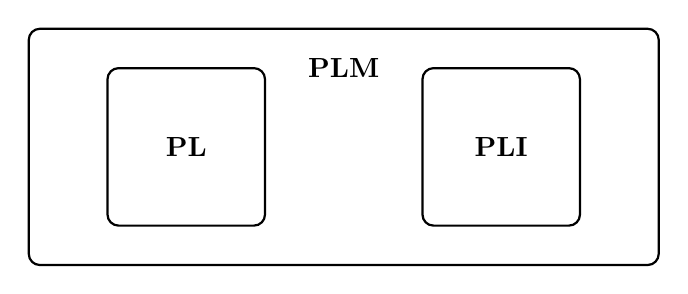
\begin{tikzpicture}
    
    \draw[thick, rounded corners] (-4, -1.5) rectangle (4, 1.5);
    
    \draw[thick, rounded corners] (-3, -1) rectangle (-1, 1);
    \node at (-2, 0) {\textbf{PL}};
    
    \draw[thick, rounded corners] (1, -1) rectangle (3, 1);
    \node at (2, 0) {\textbf{PLI}};
    
    \node at (0, 1) {\textbf{PLM}};
    
  \end{tikzpicture}
\end{center}
  
  


Un problema PL può sempre essere espresso nella seguente forma matriciale:
\[
  \max \{cx \mid Ax \leq b\}
\]
dove $ A \in \mathbb{R}^{m \times n} $ e $ b \in \mathbb{R}^m $. Grazie ad alcuni accorgimenti è possibile, inoltre, scrivere tutti i vincoli possibili di un problema di PL $\mathcal{P}$ in un'unico sistema di disequazioni lineari. Infatti:
\begin{itemize}
  \item Se \p è un problema di minimo, occorre considerare semplicemente la funzione $f (x) = (-c)x$
  \item Ogni vincolo $ax = b $diventa la coppia di vincoli $ax \leq b$ e $ax \geq b$
  \item Ogni vincolo $ax \geq b$ è equivalente a $(-a)x \leq (-b)$.
\end{itemize}

\subsection{Programmazione lineare intera}
Se nella $PL$ le variabili rappresentano quantità nella PLI le variabili possono essere
\begin{itemize}
  \item \textbf{Quantitative}: ovvero rappresentare quantità.
  \item \textbf{Logiche}: rappresentare valori booleani, ovvero scelte basate sulla possibilità di scegliere o meno una determinata opzione
\end{itemize}

Qui la definizione di variabile logica

\dfn{variabile logica}{
  Una \textbf{variabile} $x$ si definisce \textbf{logica} se:
  \[
    x \in \mathbb{N} (o \mathbb{Z}) \quad 0\leq x \quad x \leq 1
  \]
}

Un esempio tipico è rappresentato dalle variabili che associano una determinata risorsa a un compito specifico, oppure che determinano l'utilizzo di un particolare processo.

\begin{quote}
  Questo e' il bello dei problemi lineari

  \hfill -- Il Basta
\end{quote}

Un giga esempietto bellino è il problema dello zaino:
\ex{Problema dello zaino}{
  Il problema dello zaino è un esempio classico di problema di ottimizzazione combinatoria piuttosto complesso.

  % TODO: inserire il testo del problema
  TODO: inserire il testo del problema

  \vspace{1em}
  \textbf{Parametri:}
  \begin{align*}
    E &= \{1, \ldots, n\} \\
    a_i &= \text{peso dell'oggetto } i \\
    c_i &= \text{costo dell'oggetto } i \\
    b &= \text{peso massimo dello zaino}
  \end{align*}

  \vspace{1em}
  \textbf{Variabili:}
  \begin{align*}
  x_i &=
  \begin{cases}
  1 & \text{se l'oggetto } i \text{ è nello zaino} \\
  0 & \text{altrimenti}
  \end{cases} \\
  x_i &\in \{0, 1\} \quad \forall i \in \{1, \ldots, n\}
  \end{align*}

  \vspace{1em}
  \textbf{Vincoli:}
  \[
    \sum_{i=1}^{n} x_i a_i \leq b
  \]

  \vspace{1em}
  \textbf{Funzione obiettivo:}
  \[
    \max \sum_{i=1}^{n} x_i c_i
  \]

}

% Esempi di problemi di ottimizzazione lineari:
% \begin{itemize}
% \item Lo Zaino
% \item Albero di copertura minimo
% \item Commesso viaggiatore
% \end{itemize}

% \subsection{Problema dello Zaino}
% appunti scritti

\subsubsection{Relazioni logiche}

Avendo introdotto le variabili logiche, è opportuno chiedersi se sia possibile esprimere, mediante programmazione lineare (PL), le regole di inferenza logica per le relazioni che intercorrono tra di esse. Grazie all'uso di opportuni vincoli lineari, la risposta è affermativa:

\begin{itemize}
  \item \textbf{Negazione} \( (y = \neg x) \):
    \[
    x = 1 - y
    \]

  \item \textbf{Congiunzione} \( (z = x \land y) \):
    \[
    \begin{aligned}
      &z \leq x \\
      &z \leq y \\
      &z \geq x + y - 1
    \end{aligned}
    \]

  \item \textbf{Disgiunzione} \( (z = x \lor y) \):
    \[
    \begin{aligned}
      &z \geq x \\
      &z \geq y \\
      &z \leq x + y
    \end{aligned}
    \]

  \item \textbf{Implicazione} \( (z = x \implies y) \):
    \[
    \begin{aligned}
      &x + z \geq 1 \\
      &z \geq y \\
      &x + z \leq 1 + y
    \end{aligned}
    \]
\end{itemize}

È possibile, tuttavia, dimostrare che il problema di ottimizzazione lineare è, in generale, \textit{NP-hard}, dato che il problema di soddisfacibilità di una formula logica rientra nella classe NP-hard
\section{Template per risolvere problemi}

\subsection{Vincoli di assegnamento}
Un tipo di vincolo che la programmazione lineare intera (PLI) gestisce in modo molto efficace è rappresentato dai cosiddetti \textit{vincoli di assegnamento}. Questi vincoli sono utilizzati per modellare problemi che riguardano l'assegnazione di "oggetti a luoghi".

Si considerano:
\begin{itemize}
  \item Un insieme \( N = \{1, \ldots, n\} \) di \textbf{oggetti} (che possono rappresentare automezzi, persone, ecc.)
  \item Un insieme \( V = \{1, \ldots, m\} \) di \textbf{luoghi}
\end{itemize}

Per rappresentare le diverse condizioni di assegnazione degli oggetti ai luoghi, si introduce la variabile \( x_{ij} \in \{0, 1\} \) (dove \( 1 \leq i \leq n \) e \( 1 \leq j \leq m \)). Questa variabile indica se l'i-esimo oggetto è stato assegnato al j-esimo luogo (\( x_{ij} = 1 \)) o meno (\( x_{ij} = 0 \)), si può così procedere alla formale

\dfn{Vincoli di assegnamento}{
  Sia \( N = \{1, \ldots, n\} \) un insieme di oggetti e \( V = \{1, \ldots, m\} \) di luoghi, si definiscono \textbf{vincoli di assegnamento} quei vincoli che impongono che \textit{ogni oggetto sia assegnato a un solo luogo e ad ogni luogo è assegnato esattamente un oggetto}. Questi sono espressi mediante queste sommatorie:
  \[
    \sum_{j=1}^{m} x_{ij} = 1 \quad \forall i \in \{1, \ldots, n\} \quad \sum_{i=1}^{n} x_{ij} = 1 \quad \forall j \in \{1, \ldots, m\}
  \]

  Dove:
  \begin{itemize}
    \item \( x_{ij} \) è una variabile binaria che vale 1 se l'oggetto \( i \) è assegnato al luogo \( j \), e 0 altrimenti.
    \item La prima equazione assicura che ogni oggetto \( i \) sia assegnato esattamente a un luogo.
    \item La seconda equazione assicura che ogni luogo \( j \) riceva esattamente un oggetto.
  \end{itemize}
}

il luogo può anche essere visto come uno slot temporale, quindi imponiamo un certo pipeline


\subsubsection{Vincoli di semi-assegnamento}
I vincoli di semi-assegnamento sono una variante dei vincoli di assegnamento in cui non è necessario che ogni luogo riceva esattamente un oggetto, in particole si noti la seguente definizione

\dfn{Vincoli di semi-assegnamento}{
  Sia \( N = \{1, \ldots, n\} \) un insieme di oggetti e \( V = \{1, \ldots, m\} \) un insieme di luoghi. Si definiscono \textbf{vincoli di semi-assegnamento} quei vincoli che impongono che \textit{ogni oggetto sia assegnato ad al massimo un luogo}. Questi vincoli sono espressi mediante la seguente sommatoria:

  \[
  \sum_{j=1}^{m} x_{ij} \leq 1 \quad \forall i \in \{1, \ldots, n\}
  \]
  
  Dove \( x_{ij} \) è una variabile binaria che vale 1 se l'oggetto \( i \) è assegnato al luogo \( j \), e 0 altrimenti.
  

}


Insiemi ammissibili:

Vincoli di Assegnamento: ogni oggetto e' assegnato ad un luogo e ogni luogo ha un oggetto

\subsection{Selezione di Sottoinsiemi}

Sia $ N = \{1,...,n\} $ un insieme finito di elementi e sia $ F = \{F_1,...,F_n\} $ una famiglia di sottoinsiemi (non necessariamente disgiunti) dove $ F_i \subseteq N $. Vogliamo decidere qual'e' la scelta migliore di $ D\subseteq F $ di costo minimo. Per aiutare nella formulatzione del problema, possiamo rappresentare l'appartenenza degli ielementi di $ N $ in un sottoinsieme $ F_j $ come una grande matrice che ha come righe gli elementi e come colonne i sottoinsiemi. La scelta e' catturatanon piu' da $ x_{ij} $ ma solo da $ x_j $ dato che basta dire se il sottoinsieme $ j $ lo volgiamo o no. 
\[
x_j = \begin{cases}
1 & F_j \in D\\
0 & \text{altrimenti}
\end{cases}
\]

La funzione obbiettivo e' sempre:
\[
\sum_{j=1}^{n} x_j c_j
\]

I vincoli dipendono dal problema:
\begin{itemize}
\item Problema di copertura: ognuno degli eventi di $ N $ atanno in almeno uno degli elementi di $ D $:
  \[
  \sum_{j=1}^{m} a_{ij}x_j \geq 
  \]
    Numero di sottoinsiemi di $ D $ che appartengono a $ i $ (?). I sottoinsiemi $ F $ di $ N $ possono essere dei curriculum dove c'e' scritto quale dei linguaggi di programmazione $ n \in N $ conosce un candidato. Ogni candidato ha anche uno stipendio. Dobbiamo scegliere quali canditati assumere per coprire tutti i linguaggi in $ N $ minimizzando il costo.  
  \item Partizione: $ D $ deve essere una partizione di $ N $. $ N $ possono essere dei task da svolgere e gli iniemi di $ F $ sono offerte da fornitori rispetto alla risoluzione di alcuni dei task. Quindi gli inisiemi di $ D $ devono essere disgiunti perche' non vogliamo che due societa' risolvano lo stesso task. Tutto deve essere coperto una sola volta.
  \item Riempimento: si usa solo quando si vuole massimizzare. $ N $ non sono piu' incombenze o task, ma risorse da usare una volta per costruire un prodotto (elemento di $ F $). Al piu' perche' possiamo scartare qualche componente. Possiamo usare ogni elemento di $ N $ al massimo una volta. 
\end{itemize}

\ex{Problema delle Commesse}{
  Un'agenzia deve decidere come impiegare i soi $ n $ dipendenti.

  L'azienda, nell'intervallo di tempo considerato, deve evadere $ m $ commese.

  Ciascuna commessa $ j $ deve essere svolta dal sottoinsieme $ F_j \subseteq \{1,...,n\} $ dei dipendenti dell'azienda.

  Ogni commesssa, se evase, darebbe luogo ad un ricavo pari a $ r_j $.

  Ogni dipendente puo' lavorare ad una singola commessa nell'unita' di tempo.

  SVOLGIMENTO:

  e' un problema di selezione di sottoinsiemi:
  \[
  N - \{1,...,n\} \text{elementi/dipendenti}
  \]
  \[
  F = \{F_1,...,F_m\} commesse
  \]  

  VARIABILI:
  \[
  x_{j} = \begin{cases}
  1 & F_j \in D_j\\
  0 & \text{altrimenti}
  \end{cases}
  \]
  VINCOLI:
  $ 0\leq x_j \leq 1 \forall j $
  \[
  \sum_{j=1}^{m} x_j a_{ij} \leq 1 \forall i
  \]
  FO:
  \[
   \sum_{j=1}^{m} x_j r_j
 \]
 Ha fatto poi un esempio di quando c'e' una penalita' quando non fai una commessa (mi sa)
}

\subsection{Ricondurci a problemi linari}
Variabili a valori discreti possono prendere un insieme finito di valori diversi che non sono valori in un intervallo. Se questo insieme ha $ n $ valori ci servono $ n $ variabili diverse. 

\ex{Progetto di reti}{

}

alcune slide non le ho fatte

valore assoluto:
\[
  max \{f(x)| x \in X\} \quad max \{-f(x)|x \in X\}
\]
Abbiamo ridotto il problema che ha un valore assoluto a uno che non ce l'ha. Se ci fosse stata un operazione fra valori assoluti, la situa si complica

Funzioni lineari a tratti

in due dimensioni hanno la forma:
\[
  f(x) = \begin{cases}
    b_1 + c_1x & x \in [a_1, a_2]\\
    b_2+c_2x & x \in (a_2, a_3]
  \end{cases}
\]
nel punto $ a_2 $ ci puo' essere un punto di discontinuita'.

Come per il carico fisso vengono introdotte due variabili logiche asusiliarie $ y_1, y_2 $ co nil seguente significato:
\[
\]
Inoltre ci servono variabili ausiliarie che ci dicono lo spostamento rispetto a un estremo dell'intervallo a cui appartiene x:
\[
 
\]
Usiamo gli intervalli dinamici.
\[
 
\]
Non c'e' niente che ci da la funzione da ottimizzare, abbiamo solo delle definizioni che sono dei semplici commenti, i vincoli lineari sono solo gli ultimi, ma non bastano. 

Rappresentiamo la funzione $ f $ con una funzione $ g $ che prende le variabili logiche e quantitative. 
\[

\]
Il valore di $ f $ e' rappresentato univocamente dalla quadrupla, eccetto nel punto di non continuita'. Solo il primo valore e' accettabile perche' l'intervallo li e' chiuso. 

GNU MathProf





\end{document}
